\documentclass{webofc}
\usepackage[varg]{txfonts}   % Web of Conferences font
\usepackage{hyperref}
\usepackage{lineno}
%
\begin{document}
\linenumbers
%
\title{ATLAS Sim@P1 upgrades during long shutdown two}
%
\author{\firstname{Frank}
        \lastname{Berghaus}\inst{1}\fnsep\thanks{\email{berghaus@cern.ch}} \and
        \firstname{Franco} \lastname{Brasolin}\inst{2}\fnsep \and
        \firstname{Alessandro} \lastname{Di Girolamo}\inst{3}\fnsep \and
        \firstname{Marcus} \lastname{Ebert}\inst{1}\fnsep \and
        \firstname{Colin Roy} \lastname{Leavett-Brown}\inst{1}\fnsep \and
        \firstname{Chris} \lastname{Lee}\inst{4}\fnsep \and
        \firstname{Peter} \lastname{Love}\inst{5}\fnsep \and
        \firstname{Eukeni} \lastname{Pozo Astigarraga}\inst{3}\fnsep \and
        \firstname{Diana  Alessandra} \lastname{Scannicchio}\inst{6}\fnsep \and
        \firstname{Jaroslava} \lastname{Schovancova}\inst{3}\fnsep \and
        \firstname{Rolf} \lastname{Seuster}\inst{1}\fnsep \and
        \firstname{Randall}
        \lastname{Sobie}\inst{1}\fnsep\thanks{\email{sobie@uvic.ca}}
        \lastname{, on behalf of the ATLAS Collaboration}\thanks{Copyright
        [2018] CERN for the benefit of the [ATLAS Collaboration] CC-BY-4.0
        licence.}
}
%
\institute{University of Victoria, Victoria, Canada
\and
           Universit\`{a} e INFN, Bologna, Italy
\and
           CERN, Geneva, Switzerland
\and
           University of Cape Town, Cape Town, South Africa
\and
           Lancaster University, Lancaster, United Kingdom
\and
           University of California Irvine, Irvine, United States of America
          }
%
\abstract{%
  The Simulation at Point1 (Sim@P1) project was built in 2013 to take advantage
  of the ATLAS Trigger and Data Acquisition High Level Trigger (HLT) farm. The
  HLT farm provides around 100,000 cores, which are critical to ATLAS during
  data taking. When ATLAS is not recording data, such as the long shutdowns of
  the LHC, this large compute resource is  used to generate and process
  simulation data for the experiment. At the beginning of the second long
  shutdown of the large hadron collider, the HLT farm including the Sim@P1
  infrastructure was upgraded. Previous papers emphasised the need for “simple,
  reliable, and efficient tools” and assessed various options to quickly switch
  between data acquisition operation and offline processing. In this
  contribution, we describe the new mechanisms put in place for the
  opportunistic exploitation of the HLT farm for offline processing and give the
  results from the first months of operation.
}
%
\maketitle
%
\section{Introduction}
\label{intro}
ATLAS~\cite{atlas} is a general purpose experiment located at point one (P1) of
CERN's Large Hadron Collider (LHC). ATLAS employs a large computer farm,
summarised in Table~\ref{tab:hlt_hardware}, to facilitate data acquisition and
event selection.
\begin{table}
\centering
\caption{The hardware at P1 currently available for use with Sim@P1. The C6100
nodes are the decommissioned old HLT. They provide 11008 hyper-threaded (HT)
cores permanently running in offline mode. Not all cores are used to ensure the
virtual machines provide sufficient memory for ATLAS offline workloads. The
other hardware is switched to offline mode when data taking is not foreseen in
the next 24 hours. These opportunistic resources provide up to 97216 additional
cores. Usually the trigger and data acquisition team retains some resources for
their needs.}
\label{tab:hlt_hardware}
\begin{tabular}{llcccc}
\hline
Product name &
Intel\textsuperscript{\textregistered} Xeon\textsuperscript{\textregistered} &
HT cores & Memory [GB] & Instance cores & Nodes \\\hline
C6100 & X5650 & 24 & 24 & 16 & 688\\
Centerprise & E5-2650 v4 & 48 & 64 & 48 & 360 \\
Persy & E5-2660 v4 & 56 & 64 & 56 & 440 \\
MegWare & E5-2680 v3 & 48 & 64 & 48 & 680 \\
QuantaPlex & E5-2680 v3 & 48 & 64 & 48 & 472\\\hline
\end{tabular}
\end{table}
The HLT is a mission critical part of the ATLAS experiment and is physically
connected to the control network of the detector and the ``data'' network which
allows connections to the CERN data centre through a switch at
P1~\cite{tdaq2013}. The Sim@P1 project aims to opportunistically use the trigger
and data acquisition high level trigger resources for offline computing. When
working with Sim@P1 it is important to ensure the secure isolation from the
physical resources at P1, seamless integration into the ATLAS distributed
computing system, and reliable transition between the functions of the
resources. Throughout this text we will refer to standard operation of the HLT
as \textit{online mode} and the operation as part of the ATLAS distributed
computing system as \textit{offline mode}.

A system satisfying these criteria was developed during the first long shutdown
of the LHC~\cite{Ballestrero:2015ypa}. Isolation is achieved by running virtual
machines on the physical HLT hardware. The virtual machines were originally
managed using the cloud framework OpenStack~\cite{openstack}. The virtual
machines shared the ``data'' connection of the HLT hardware through a tagged
virtual local area network (VLAN), which provided network isolation on the level
of the Ethernet frame managed by the switches. This VLAN allowed the virtual
machines to connect to a controlled list of interfaces in the CERN general
purpose network. This list specifies the interface of the machines needed to
allow offline workloads to be delivered and executed. To minimise impact of
Sim@P1 on the Trigger and Data Acquisition (TDAQ) operation, only simulation
tasks from the central production system are submitted to run at P1.

The original implementation of Sim@P1 ran successfully during the first long
shutdown of the LHC facilities between 2013 and 2015. Once the experiment
resumed data-taking, the system was used
opportunistically~\cite{Ballestrero:2017psv}. The HLT was switched from TDAQ
function to offline mode for intervals of a few days during technical stops and
machine development. To allow this opportunistic usage a set of scripts were
developed to manage the transition of resources between online and offline
function.

During the second long shutdown of the LHC facilities, starting in 2019, the HLT
was upgraded. The changes to the HLT necessitated an upgrade of the Sim@P1
infrastructure\footnote{The Icehouse release of OpenStack does not support
CentOS7, which started running on the HLT in 2019.}. A previous
publication offered multiple options for this upgrade~\cite{Berghaus:2019wuj}.
In this paper, we describe how the system was modified for operation with the
upgraded HLT hardware.

\section{The Sim@P1 infrastructure}
\label{sec:infra}
During the year end technical stop from December 2017 to March 2018, the
computing hardware of the HLT was replaced with new nodes. Some old HLT hardware
was retained at P1 and is permanently operating in offline mode. The new
hardware has been used offline during the various technical and machine
development stops throughout 2018. The current hardware configuration is
summarised in Table~\ref{tab:hlt_hardware}. Groups of 32 or 40 servers are
organised into racks in the data centre at P1.

When a rack is not needed for data taking a shifter can set that rack to
offline operation. This action triggers a change in the configuration database
used by the TDAQ. The next time the configuration management system runs on any
server, or trigger processing unit (TPU), in that rack\footnote{The
configuration management tool, Puppet, runs once an hour on the TPUs.} it
changes the system configuration to reflect the change in the configuration
database. An ephemeral disk providing 20\,\textrm{GB} per core is
created and a virtual machine instance is started\footnote{The size of the
ephemeral disk is reduced to ensure at least 20\% of the hard drive is free.}.
This document will refer to such a running virtual machine as an
\textit{instance}.

Instances are contextualised using amiconfig\footnote{Originally a
project by rPath, Inc. now maintained by the CernVM team.}~\cite{amiconfig}.
The contextualisation is delivered using an ISO image added to the instance
by libvirt~\cite{libvirt}. The ISO image is formatted as an OpenNebula data
source. The contextualisation sets up the computing environment for the ATLAS
offline workloads and sets the virtual machines to advertise themselves to a
HTCondor system running in the CERN general purpose network~\cite{condor}.
Instances are configured to use HTCondor's dynamic partitioning feature to
map workloads to the resources. Process isolation is achieved using the control
groups feature of the Linux kernel.

The HTCondor system for Sim@P1 was rebuilt with a single central manager and
four schedulers. The virtual machines are managed by CERN's configuration
management system. Work is submitted to the schedulers using the PanDA
Harvester~\cite{harvester}. Sim@P1 presents a single unified production queue to
the PanDA system. The Harvester is operating the queue in push mode allowing the
workloads to request the resources they need leveraging the dynamic partitioning
of workers.  The HTCondor system now directly notifies the PanDA workload
management system when resources are added or removed from Sim@P1.

The new Sim@P1 network configuration still uses tags in the Ethernet frames to
isolate traffic on a VLAN. Network security is improved by using a virtual
router\footnote{With a separate IP table.} that manages only traffic in that
VLAN. This avoids traffic being forwarded to an unintended host by accident.
Furthermore, the online traffic is given a higher quality of service guarantee
than traffic on the Sim@P1 VLAN. That means offline activities can potentially
receive the full bandwidth available on the network, but will never impact
traffic from other TDAQ activities - such as data taking.

\subsection{Content delivery}
CernVM is a good solution for Sim@P1 because the micro-image can be distributed
to all the TPUs and require a trivial disk space during HLT operation. Using
CernVM means that we rely on the CernVM file system (CVMFS) to provide both the
operating system content as well as the experiment software. In our CHEP2018
contribution we incorrectly stated that the load on the Frontier squids during
the switch to offline mode was low~\cite{Berghaus:2019wuj, Dykstra:2019}.
This measurement was flawed: the instances were incorrectly contextualised to
retrieve the CVMFS content from the Frontier squids operated by CERN IT for
their batch system. Figure~\ref{fig:single_proxy} shows that, after correcting
the contextualisation, the Frontier squid at P1 was saturating its network
bandwidth to deliver the content required by the booting instances.
\begin{figure}[h]
\centering
\sidecaption
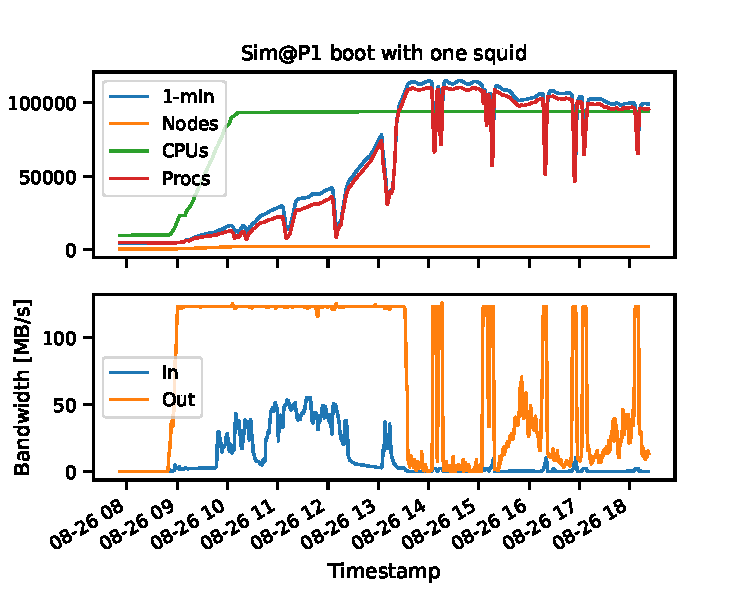
\includegraphics[width=0.6\textwidth,clip]{single_squid}
\caption{The top figure shows the number of instances, CPUs, and running
processes as well as the aggregate one minute load on the TDAQ HLT farm as it
transitions to offline mode. Below, using the same timestamps, the network load
on the single Frontier proxy delivering the CVMFS content to all the nodes is
displayed. The correlation of saturated outgoing bandwidth in the lower plot
with
the steady increase in the load and processes in the upper plot suggests the
squid is the rate determining system in the transition of the farm.}
\label{fig:single_proxy}
\end{figure}
To address the bottleneck posed by the single squid we added a second squid
instance, then added CVMFS caches that persist throughout HLT operation, and
finally created a hierarchy of squids on the instances in offline mode.

The addition of a second squid doubled the total bandwidth used to deliver the
content required for CVMFS. As a result the transition to offline mode finished
in three hours: approximately twice as fast as with the single Frontier squid.


\subsection{Persistent CVMFS caches}
\label{sec:cvmfs}
Much of the CVMFS content remains unchanged between successive switches between
offline and online mode: changes to the files in the CernVM system tend to be
minimal and an ATLAS software release once downloaded does not change. So
keeping the CVMFS cache throughout online operation reduces the
amount of content the caches need to provide when transitioning to offline mode.

A $50$\,\textrm{GB} virtual disk image was created on each TPU to serve as
persistent CVMFS cache. The ephemeral disk may be smaller to
compensate for the size of the cache. Libvirt is configured to mount the cache
as an additional drive. The contextualisation checks for a second drive. If it
finds the second disk exists and is formatted with the label ``cache'' it
mounts the disk as the CVMFS cache. If the second disk exists but carries no
labelled partition the disk is formatted with the label ``cache'' and mounted.

Figure~\ref{fig:persistent_cache} shows that with a warm CVMFS cache the farm
boots in an hour, with a slight time delay between the virtual machine being
created and being fully occupied with work.
\begin{figure}[h]
\centering
\sidecaption
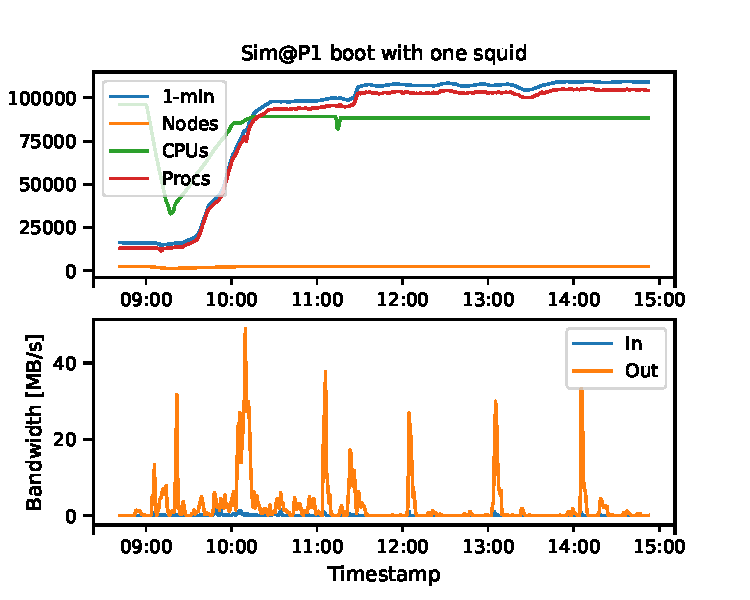
\includegraphics[width=0.6\textwidth,clip]{persistent_cache}
\caption{The top figure shows the number of instances, CPUs, and running
processes as well as the aggregate one minute load on the TDAQ HLT farm as it
transitions to offline mode. Below, using the same timestamps, the network load
on the two Frontier squids delivering the CVMFS content to all the nodes is
displayed. With the persistent cache the network traffic on the squids
is greatly reduced.}
\label{fig:persistent_cache}
\end{figure}


\subsection{Squid hierarchy}
\label{sec:hierarchy}
The contextualisation of the instances was adjusted to run a squid in two
instances in each rack, as a complimentary approach to the persistent CVMFS
caches\footnote{The first and fifth TPU to ensure the squids are in
separate chassis.}. The squids treat each other as siblings and the Frontier
squid caches at P1 as parents. A web proxy-autodiscovery service is set up to
connect virtual machines to proxy caches on boot: those serving a squid
connect to the central Frontier squids at P1, others are connected to the two
squids in the same rack. The CernVM team added functionality to the CernVM
micro-kernel to delay the boot process until at least one proxy cache is up.


\section{Operational experience}
\label{sec:ops}
The new configuration of Sim@P1 was operational within two days of the upgrade
to the TDAQ HLT. This quick transition is a testament to the simplification of
the Sim@P1 infrastructure under the new configuration. A feature of libvirt
which negatively effects returning the resources to online operation was
discovered. The following section described the workaround that was implemented.
The squid hierarchy provided a marginal improvement in the transition from
online to offline operation while reducing the overall stability of the system:
we started loosing racks when the two squids in the rack cease functioning.

\subsection{Returning the resources}
\label{sec:return}
Returning the resource to online mode quickly and reliably is absolutely
essential, more so when ATLAS is taking data. Should an instance running on a
TPU be busy with IO intensive work, it may take time O(10\,\textrm{s}) for
libvirt to destroy the instance\footnote{Usually an active application using
swap space.}. Libvirt has a timeout of 15\,\textrm{s} waiting on the destruction
of a virtual machine, taking longer produces an error in returning that TPU to
online mode. A helper script to manage the instance state was written. It
attempts to destroy the instance three times, with a 15\,\textrm{s} delay between
attempts. With this modification, all resources were successfully returned to
online mode without issues.

\subsection{Other workflows}
\label{sec:evgen}
Data taken by ATLAS is cached at P1 and transferred to the CERN data
centre. Tests performed at the end of 2018 have shown that we must assume the
network between point 1 and CERN to be busy transferring data from the cache to
storage in the CERN data centre during technical stops. Offline operation must
not interfere with the process. That means workflows requiring little data
transfer across the network, such as simulation, are a natural fit for Sim@P1.

Event generation is a frequent task that requires no input and produces very
little output. Previous experience with event generation found that depending on
the software used and the physics signal generated these tasks have a long tail
in the required memory. We created dedicated high memory and single core queues
to explore the use of Sim@P1 for event generation. At the end of 2019, the first
event generation tasks were successfully executed on Sim@P1. Since event
generation in ATLAS is a workload using a single core, the four HTCondor
schedulers were fully occupied managing event generation reducing the overall
usage of Sim@P1.

\subsection{Future improvements}
The infrastructure supporting Sim@P1 could be further improved to reduce the
work required to maintain and operate the resource.

The success in running event generation in late 2019 shows that this could be
done in an automated setup. However workloads that greatly exceeding their
memory allocation must be killed by HTCondor to ensure system stability. In
addition, additional HTCondor schedulers must be commissioned to accommodate the
increased number of jobs and limit the number of single core jobs allowed in the
queue.

The hardware serving as Frontier squids operating at P1 needs to be replaced.
Supporting greater bandwidth for the CVMFS and Frontier content distribution
will further improve the rate at which the farm can be switched from online to
offline mode. New hardware would mean the squid hierarchy described in
section~\ref{sec:hierarchy} could be removed, improving the stability of Sim@P1.

As longer term project, OpenStack Heat or Kubernetes could be used to build
and auto-scaling pool of HTCondor schedulers. Adding volatile storage to
serve as a cache inside P1 may allow more data hungry workflows to be executed
without interfering with online operations\footnote{Such as Xcache or a volatile
Disk Pool Manager.}.

\section{Conclusions}
The TDAQ HLT of the ATLAS experiment at the LHC was upgraded at the beginning of
2019. The infrastructure for the opportunistic usage of this large computing
resource, Sim@P1, was swiftly and successfully configured to function on the
updated HLT hardware. This new configuration is simpler and more robust: it
relies on low level Linux tools and systems maintained by the
TDAQ administrators. The system has become much more responsive by adding
persistent CVMFS caches. Future improvements promise to make Sim@P1 more robust,
versatile and easy to manage.


\begin{thebibliography}{}
  \bibitem{atlas}
   The ATLAS Collaboration,
   %The  ATLAS  Experiment  at  the  CERN  Large  Hadron  Collider,
   JINST \textbf{3}, S08003 (2008)
   \url{https://doi.org/10.1088/1748-0221/3/08/S08003}
   \doi{10.1088/1748-0221/3/08/S08003}

  \bibitem{tdaq2013}
    The ATLAS Collaboration, \textit{Technical Design Report for the Phase-I
    Upgrade of the ATLAS TDAQ System} (CERN, Geneva, 2013) 120-122
    \url{https://cds.cern.ch/record/1602235}

  \bibitem{Ballestrero:2015ypa}
    S.~Ballestrero \textit{et al},
    J.\ Phys.\ Conf.\ Ser.\  \textbf{664}, 2 022008 (2015)
    \url{https://doi.org/10.1088/1742-6596/664/2/022008}
    \doi{10.1088/1742-6596/664/2/022008}

  \bibitem{openstack}
    Openstack project, ”OpenStack” [software], version Icehouse, available from
    \url{https://www.openstack.org/software/icehouse/} [accessed 2018-09-24]

  \bibitem{Ballestrero:2017psv}
    S.~Ballestrero \textit{et al},
    %``Evolution and experience with the ATLAS Simulation at Point1 Project,''
    J.\ Phys.\ Conf.\ Ser.\  \textbf{898},  8 082012 (2017)
    \url{https://doi.org/10.1088/1742-6596/898/8/082012}
    \doi{10.1088/1742-6596/898/8/082012}

  \bibitem{Berghaus:2019wuj}
    F.~Berghaus \textit{et al} [ATLAS Collaboration],
    EPJ Web Conf.\ \textbf{214}, 07021 (2019)
    \url{https://doi.org/10.1051/epjconf/201921407021}
    \doi{10.1051/epjconf/201921407021}

  \bibitem{amiconfig}
    CernVM project, ``amiconfig'' [software], available from
    \url{https://github.com/cernvm/amiconfig} [accessed 2018-10-10]

  \bibitem{libvirt}
    libvirt project, ``libvirt virtualization API'' [software], version 0.10.2,
    available from \url{https://libvirt.org} [accessed 2018-10-10]

  \bibitem{condor}
    D. Thain, T. Tannenbaum and M. Livny,
    % Distributed computing in practice: the Condor experience,
    Concurrency and Computation: Practice and Experience \textbf{17} 323-356
    (2005)
    \url{https://doi.org/10.1002/cpe.938}
    \doi{10.1002/cpe.938}

  \bibitem{harvester}
    T. Maeno \textit{et al} [ATLAS Collaboration],
    % Harvester : an edge service harvesting heterogeneous resources for ATLAS
    EPJ Web of Conf.\ \textbf{214}, 03030 (2019)
    \url{https://doi.org/10.1051/epjconf/201921403030}
    \doi{10.1051/epjconf/201921403030}

  \bibitem{Dykstra:2019}
    Frontier project, ``Frontier squid'' [software], available from
    \url{https://twiki.cern.ch/twiki/bin/view/Frontier/InstallSquid}
    [accessed 2020-01-17]

  \bibitem{cernvm}
    J. Blomer \textit{et al},
    %Micro-CernVM: slashing the cost of building and deploying virtual machines,
    J.\ Phys.: Conf.\ Ser.\ \textbf{513} 032009 (2014)
    \url{https://doi.org/10.1088/1742-6596/513/3/032009}
    \doi{10.1088/1742-6596/513/3/032009}

\end{thebibliography}

\end{document}
